\documentclass{standalone}
\usepackage{tikz}
\usetikzlibrary{patterns, positioning}


\begin{document}
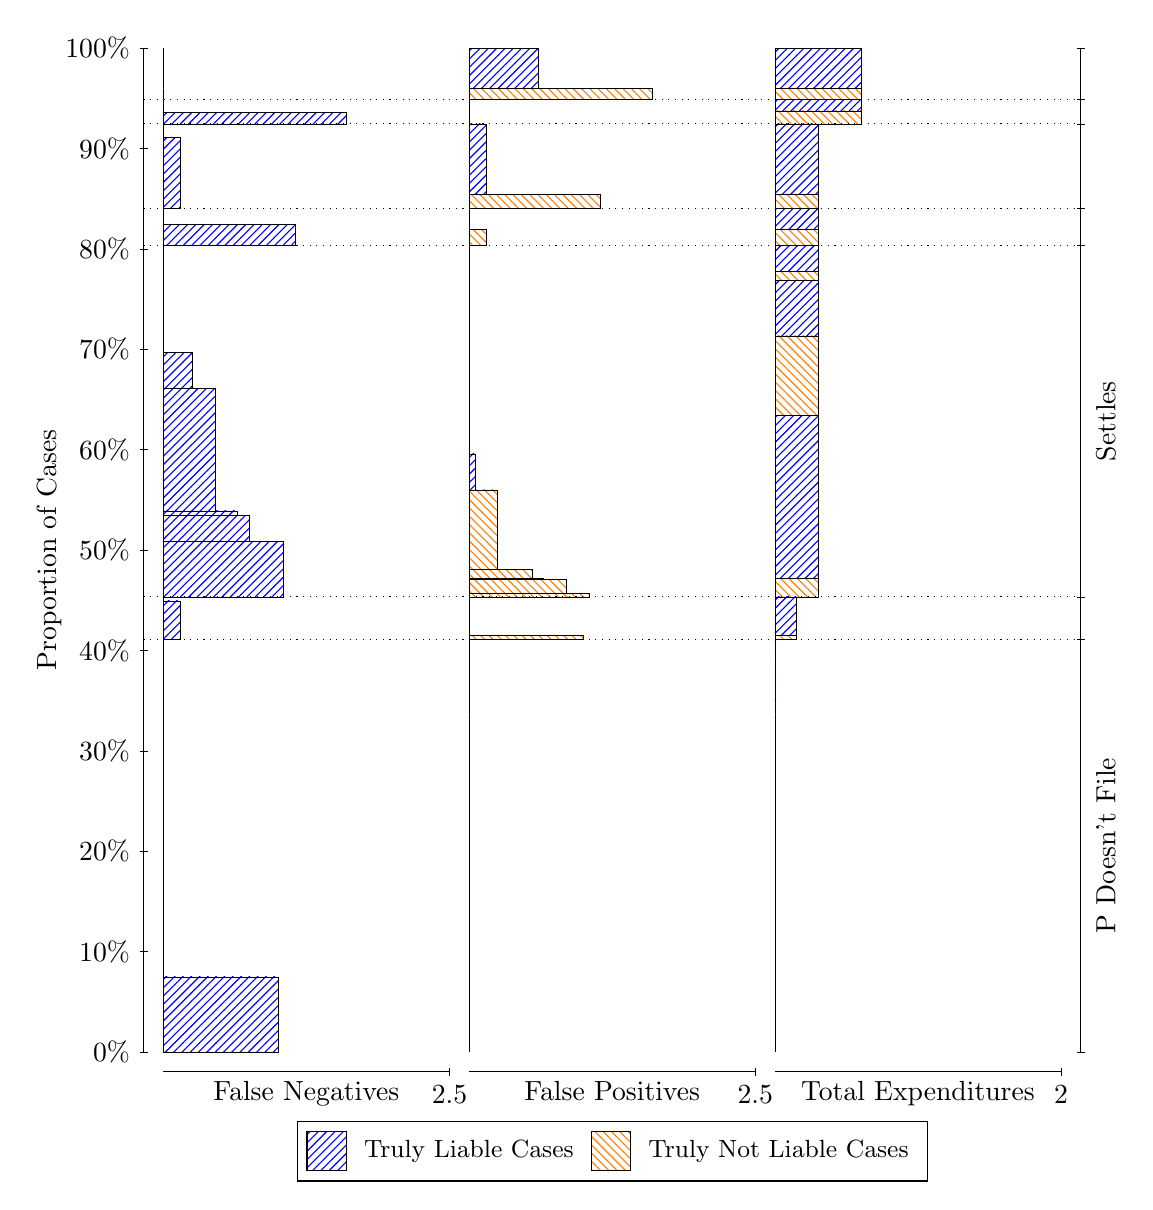
\begin{tikzpicture}
\draw[black, very thin] (1.5,1.75) -- (1.5,14.5);
\node[rotate=90, text=black, anchor=center] at (0.3, 8.125) {Proportion of Cases};
\draw[black, very thin] (1.45,1.75) -- (1.55,1.75);
\node[text=black, anchor=east] at (1.45, 1.75) {0\%};
\draw[black, very thin] (1.45,3.025) -- (1.55,3.025);
\node[text=black, anchor=east] at (1.45, 3.025) {10\%};
\draw[black, very thin] (1.45,4.3) -- (1.55,4.3);
\node[text=black, anchor=east] at (1.45, 4.3) {20\%};
\draw[black, very thin] (1.45,5.575) -- (1.55,5.575);
\node[text=black, anchor=east] at (1.45, 5.575) {30\%};
\draw[black, very thin] (1.45,6.85) -- (1.55,6.85);
\node[text=black, anchor=east] at (1.45, 6.85) {40\%};
\draw[black, very thin] (1.45,8.125) -- (1.55,8.125);
\node[text=black, anchor=east] at (1.45, 8.125) {50\%};
\draw[black, very thin] (1.45,9.4) -- (1.55,9.4);
\node[text=black, anchor=east] at (1.45, 9.4) {60\%};
\draw[black, very thin] (1.45,10.675) -- (1.55,10.675);
\node[text=black, anchor=east] at (1.45, 10.675) {70\%};
\draw[black, very thin] (1.45,11.95) -- (1.55,11.95);
\node[text=black, anchor=east] at (1.45, 11.95) {80\%};
\draw[black, very thin] (1.45,13.225) -- (1.55,13.225);
\node[text=black, anchor=east] at (1.45, 13.225) {90\%};
\draw[black, very thin] (1.45,14.5) -- (1.55,14.5);
\node[text=black, anchor=east] at (1.45, 14.5) {100\%};

\draw[black, very thin] (13.4,1.75) -- (13.4,14.5);
\draw[black, very thin] (13.35,1.75) -- (13.45,1.75);
\node[anchor=west] at (13.35, 1.75) {};
\draw[black, very thin] (13.35,6.9893) -- (13.45,6.9893);
\node[anchor=west] at (13.35, 6.9893) {};
\draw[black, very thin] (13.35,7.5296) -- (13.45,7.5296);
\node[anchor=west] at (13.35, 7.5296) {};
\draw[black, very thin] (13.35,11.994) -- (13.45,11.994);
\node[anchor=west] at (13.35, 11.994) {};
\draw[black, very thin] (13.35,12.465) -- (13.45,12.465);
\node[anchor=west] at (13.35, 12.465) {};
\draw[black, very thin] (13.35,13.538) -- (13.45,13.538);
\node[anchor=west] at (13.35, 13.538) {};
\draw[black, very thin] (13.35,13.844) -- (13.45,13.844);
\node[anchor=west] at (13.35, 13.844) {};
\draw[black, very thin] (13.35,14.5) -- (13.45,14.5);
\node[anchor=west] at (13.35, 14.5) {};

\draw[black, very thin, pattern color=blue, pattern=north east lines] (1.75,1.75) rectangle (3.2033,2.7039);
\draw[black, very thin, pattern color=orange, pattern=north west lines] (1.75,2.7039) rectangle (1.75,6.9893);
\draw[black, very thin, pattern color=blue, pattern=north east lines] (1.75,6.9893) rectangle (1.968,7.4798);
\draw[black, very thin, pattern color=orange, pattern=north west lines] (1.75,7.4798) rectangle (1.75,7.5296);
\draw[black, very thin, pattern color=blue, pattern=north east lines] (1.75,7.5296) rectangle (3.276,8.2339);
\draw[black, very thin, pattern color=blue, pattern=north east lines] (1.75,8.2339) rectangle (2.84,8.5642);
\draw[black, very thin, pattern color=blue, pattern=north east lines] (1.75,8.5642) rectangle (2.6947,8.623);
\draw[black, very thin, pattern color=blue, pattern=north east lines] (1.75,8.623) rectangle (2.404,10.177);
\draw[black, very thin, pattern color=blue, pattern=north east lines] (1.75,10.177) rectangle (2.1133,10.634);
\draw[black, very thin, pattern color=orange, pattern=north west lines] (1.75,10.634) rectangle (1.75,11.994);
\draw[black, very thin, pattern color=blue, pattern=north east lines] (1.75,11.994) rectangle (3.4213,12.265);
\draw[black, very thin, pattern color=orange, pattern=north west lines] (1.75,12.265) rectangle (1.75,12.465);
\draw[black, very thin, pattern color=blue, pattern=north east lines] (1.75,12.465) rectangle (1.968,13.364);
\draw[black, very thin, pattern color=orange, pattern=north west lines] (1.75,13.364) rectangle (1.75,13.538);
\draw[black, very thin, pattern color=blue, pattern=north east lines] (1.75,13.538) rectangle (4.0753,13.68);
\draw[black, very thin, pattern color=orange, pattern=north west lines] (1.75,13.68) rectangle (1.75,13.844);
\draw[black, very thin, pattern color=orange, pattern=north west lines] (1.75,13.844) rectangle (1.75,13.987);
\draw[black, very thin, pattern color=blue, pattern=north east lines] (1.75,13.987) rectangle (1.75,14.5);
\draw[black, very thin, pattern color=orange, pattern=north west lines] (5.6333,1.75) rectangle (5.6333,6.0354);
\draw[black, very thin, pattern color=blue, pattern=north east lines] (5.6333,6.0354) rectangle (5.6333,6.9893);
\draw[black, very thin, pattern color=orange, pattern=north west lines] (5.6333,6.9893) rectangle (7.0867,7.0391);
\draw[black, very thin, pattern color=blue, pattern=north east lines] (5.6333,7.0391) rectangle (5.6333,7.5296);
\draw[black, very thin, pattern color=orange, pattern=north west lines] (5.6333,7.5296) rectangle (7.1593,7.5696);
\draw[black, very thin, pattern color=orange, pattern=north west lines] (5.6333,7.5696) rectangle (6.8687,7.7517);
\draw[black, very thin, pattern color=orange, pattern=north west lines] (5.6333,7.7517) rectangle (6.578,7.764);
\draw[black, very thin, pattern color=orange, pattern=north west lines] (5.6333,7.764) rectangle (6.4327,7.8777);
\draw[black, very thin, pattern color=orange, pattern=north west lines] (5.6333,7.8777) rectangle (5.9967,8.8892);
\draw[black, very thin, pattern color=blue, pattern=north east lines] (5.6333,8.8892) rectangle (5.706,9.3467);
\draw[black, very thin, pattern color=blue, pattern=north east lines] (5.6333,9.3467) rectangle (5.6333,11.994);
\draw[black, very thin, pattern color=orange, pattern=north west lines] (5.6333,11.994) rectangle (5.8513,12.193);
\draw[black, very thin, pattern color=blue, pattern=north east lines] (5.6333,12.193) rectangle (5.6333,12.465);
\draw[black, very thin, pattern color=orange, pattern=north west lines] (5.6333,12.465) rectangle (7.3047,12.638);
\draw[black, very thin, pattern color=blue, pattern=north east lines] (5.6333,12.638) rectangle (5.8513,13.538);
\draw[black, very thin, pattern color=orange, pattern=north west lines] (5.6333,13.538) rectangle (5.6333,13.702);
\draw[black, very thin, pattern color=blue, pattern=north east lines] (5.6333,13.702) rectangle (5.6333,13.844);
\draw[black, very thin, pattern color=orange, pattern=north west lines] (5.6333,13.844) rectangle (7.9587,13.987);
\draw[black, very thin, pattern color=blue, pattern=north east lines] (5.6333,13.987) rectangle (6.5053,14.5);
\draw[black, very thin, pattern color=orange, pattern=north west lines] (9.5167,1.75) rectangle (9.5167,6.0354);
\draw[black, very thin, pattern color=blue, pattern=north east lines] (9.5167,6.0354) rectangle (9.5167,6.9893);
\draw[black, very thin, pattern color=orange, pattern=north west lines] (9.5167,6.9893) rectangle (9.7892,7.0391);
\draw[black, very thin, pattern color=blue, pattern=north east lines] (9.5167,7.0391) rectangle (9.7892,7.5296);
\draw[black, very thin, pattern color=orange, pattern=north west lines] (9.5167,7.5296) rectangle (10.062,7.764);
\draw[black, very thin, pattern color=blue, pattern=north east lines] (9.5167,7.764) rectangle (10.062,9.834);
\draw[black, very thin, pattern color=orange, pattern=north west lines] (9.5167,9.834) rectangle (10.062,10.845);
\draw[black, very thin, pattern color=blue, pattern=north east lines] (9.5167,10.845) rectangle (10.062,11.55);
\draw[black, very thin, pattern color=orange, pattern=north west lines] (9.5167,11.55) rectangle (10.062,11.663);
\draw[black, very thin, pattern color=blue, pattern=north east lines] (9.5167,11.663) rectangle (10.062,11.994);
\draw[black, very thin, pattern color=orange, pattern=north west lines] (9.5167,11.994) rectangle (10.062,12.193);
\draw[black, very thin, pattern color=blue, pattern=north east lines] (9.5167,12.193) rectangle (10.062,12.465);
\draw[black, very thin, pattern color=orange, pattern=north west lines] (9.5167,12.465) rectangle (10.062,12.638);
\draw[black, very thin, pattern color=blue, pattern=north east lines] (9.5167,12.638) rectangle (10.062,13.538);
\draw[black, very thin, pattern color=orange, pattern=north west lines] (9.5167,13.538) rectangle (10.607,13.702);
\draw[black, very thin, pattern color=blue, pattern=north east lines] (9.5167,13.702) rectangle (10.607,13.844);
\draw[black, very thin, pattern color=orange, pattern=north west lines] (9.5167,13.844) rectangle (10.607,13.987);
\draw[black, very thin, pattern color=blue, pattern=north east lines] (9.5167,13.987) rectangle (10.607,14.5);
\draw[black, dotted] (1.5,6.9893) -- (13.4,6.9893);
\draw[black, dotted] (1.5,7.5296) -- (13.4,7.5296);
\draw[black, dotted] (1.5,11.994) -- (13.4,11.994);
\draw[black, dotted] (1.5,12.465) -- (13.4,12.465);
\draw[black, dotted] (1.5,13.538) -- (13.4,13.538);
\draw[black, dotted] (1.5,13.844) -- (13.4,13.844);
\draw[black, very thin] (1.75,1.5) -- (5.3833,1.5);
\node[text=black, anchor=north] at (3.5667, 1.5) {False Negatives};
\draw[black, very thin] (5.3833,1.45) -- (5.3833,1.55);
\node[text=black, anchor=north] at (5.3833, 1.45) {2.5};

\draw[black, very thin] (5.6333,1.5) -- (9.2667,1.5);
\node[text=black, anchor=north] at (7.45, 1.5) {False Positives};
\draw[black, very thin] (9.2667,1.45) -- (9.2667,1.55);
\node[text=black, anchor=north] at (9.2667, 1.45) {2.5};

\draw[black, very thin] (9.5167,1.5) -- (13.15,1.5);
\node[text=black, anchor=north] at (11.333, 1.5) {Total Expenditures};
\draw[black, very thin] (13.15,1.45) -- (13.15,1.55);
\node[text=black, anchor=north] at (13.15, 1.45) {2};

\node[text=black, centered, rotate=90] at (13.72, 4.3697) {P Doesn't File};

\node[text=black, centered, rotate=90] at (13.72, 9.7617) {Settles};





\draw (7.449999999999999,1.5) node[draw=none] (baseCoordinate) {};
\begin{scope}[align=center]
        \matrix[scale=0.5, draw=black, below=0.5cm of baseCoordinate, nodes={draw}, column sep=0.1cm]{
            \node[rectangle, draw, minimum width=0.5cm, minimum height=0.5cm, pattern color=blue, pattern=north east lines] {}; &
            \node[draw=none, font=\small, text=black] (B) {Truly Liable Cases}; &
            \node[rectangle, draw, minimum width=0.5cm, minimum height=0.5cm, pattern color=orange, pattern=north west lines] {}; &
            \node[draw=none, font=\small, text=black] (B) {Truly Not Liable Cases}; \\
            };
\end{scope}

\end{tikzpicture}
\end{document}